\subsection{Synchronization}

The following section has been enhanced with slides from Senior Principal Engineer Mattson Tim. He's a senior principal engineer at Intel, where he's been since 1993. His profile can be seen \href{https://www.intel.com/content/www/us/en/research/featured-researchers/tim-mattson.html}{here} and the slides are available online \href{https://www.openmp.org/wp-content/uploads/Intro_To_OpenMP_Mattson.pdf}{here}. He has also made an interesting \href{https://youtube.com/playlist?list=PLLX-Q6B8xqZ8n8bwjGdzBJ25X2utwnoEG&si=OBjyY4AI4zWfA-vB}{YouTube series} on the introduction to OpenMP.

\highspace
OpenMP is a multi-threaded, shared address model. This means that threads communicate by sharing variables. Unfortunately, this can cause some problems such as race conditions (page \pageref{def: race condition}). The solution is to \textbf{use synchronization to protect against data conflicts}. The good news is that synchronization can avoid data race problems, but it is also an \textbf{expensive method}. So we can use synchronization, but we \textbf{need to change the way data is accessed to minimize the need for synchronization}.

\highspace
Synchronization brings \textbf{one or more threads to a well-defined and known point in their execution}. The two most common forms of synchronization are:
\begin{itemize}
    \item \textbf{\emph{Barrier}}: each thread wait at the barrier \textbf{until all threads arrive}.
    \item \textbf{\emph{Mutual exclusion}}: define a block of code that \textbf{only one thread at a time can execute}.
\end{itemize}
The OpenMP directives are: \texttt{critical}, \texttt{atomic}, and \texttt{barrier}. These are high-level synchronization directives, but there are also low-level synchronization directives, such as \texttt{flush} and \texttt{locks}, but they are too complex at the moment, we will see them later.

\begin{figure}[!htp]
    \centering
    \begin{subfigure}{.45\textwidth}
        \centering
        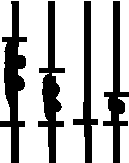
\includegraphics[width=.25\textwidth]{img/openmp-sync-1.pdf}
        \caption{Barrier. Each thread wait at the barrier until all threads arrive.}
    \end{subfigure}
    \hfill
    \begin{subfigure}{.45\textwidth}
        \centering
        
\includegraphics[width=.25\textwidth]{img/openmp-sync-2.pdf}
        \caption{Mutual exclusion. Define a block of code that only one thread at a time can execute.}
    \end{subfigure}
\end{figure}

\newpage

\noindent
\textbf{\underline{Barrier}}. Each thread waits until all threads arrive.
\begin{openmpbox}[: \texttt{barrier}]
    \begin{lstlisting}[language=C++, mathescape=true]
#pragma omp barrier $\emph{name}$\end{lstlisting}
\end{openmpbox}

\noindent
An \underline{optional} \texttt{name} may be used to identify the \texttt{critical} region. A \textbf{thread waits at the beginning of a critical region} until no other thread is executing a critical region (anywhere in the program) \textbf{with the same name}. \textbf{All unnamed \texttt{critical} directives map to the same unspecified name}.

\begin{examplebox}[: synchronization with \texttt{barrier} directive]
    The following example includes several critical directives. The example illustrates a queuing model in which a task is dequeued and worked on. To guard against many threads dequeuing the same task, the dequeuing operation must be in a \texttt{critical} section. Because the two queues in this example are independent, they're protected by \texttt{critical} directives with different names, \emph{xaxis} and \emph{yaxis}.\cite{openMPCriticalDirectiveMicrosoftExample}
    \begin{lstlisting}[language=C++]
#pragma omp parallel shared(x, y) private(x_next, y_next)
{
    #pragma omp critical ( xaxis )
        x_next = dequeue(x);
    work(x_next);
    #pragma omp critical ( yaxis )
        y_next = dequeue(y);
    work(y_next);
}
    \end{lstlisting}
\end{examplebox}

\highspace
\textbf{\underline{Mutual exclusion}}. Only one thread at a time can enter a \emph{critical} region.
\begin{openmpbox}[: \texttt{critical}]
    \begin{lstlisting}[language=C++]
#pragma omp critical\end{lstlisting}
\end{openmpbox}
\begin{table}[!htp]
    \centering
    \begin{tabular}{@{} p{8em} | p{12em} | p{12em} @{}}
        \toprule
        & \texttt{omp critical} & \texttt{omp single} \\
        \midrule
        Meaning & Run code segment one by one by all threads & Run code segment once by any thread \\
        \cmidrule{1-3}
        Number of times code is executed & Number of threads & Only one \\
        \cmidrule{1-3}
        Use case & Avoid race condition & Manage control variables or signals \\
        \bottomrule
    \end{tabular}
    \caption{\textcolor{Red2}{\faIcon{exclamation-triangle} \textbf{\texttt{omp critical} vs \texttt{omp single}}}}
\end{table}
\begin{examplebox}[: synchronization with \texttt{critical} directive]
    Note the following code:
    \begin{lstlisting}[language=C++, mathescape=true]
float res;

#pragma omp parallel
{
    float B;
    int i, id, nthrds, niters = $\emph{big\_number}$;

    id = omp_get_thread_num();
    nthrds = omp_get_num_threads();
    for (i = id; i < niters; i += nthrds) {
        B = big_job(i);
        #pragma omp critical // threads wait their turn;
        res += consume(B);   // only one at a time
    }                        // calls consume
}
    \end{lstlisting}
\end{examplebox}

\highspace
\textbf{\underline{Atomic}}. Provides mutual exclusion, but only when updating a memory location. It \textbf{ensures that a particular memory location is accessed atomically}. It is \textbf{valid only for the following statement} and not for a structured block.

\highspace
The statement inside the atomic must be one of the following forms:
\begin{itemize}
    \item \texttt{x binop = expr}
    \item \texttt{x++} or \texttt{++x}
    \item \texttt{x-}\texttt{-} or \texttt{-}\texttt{-x}
\end{itemize}
Where \texttt{x} is an lvalue of scalar type and \texttt{binop} is a non-overloaded builtin operator.

\begin{openmpbox}[: \texttt{atomic}]
    \begin{lstlisting}[language=C++]
#pragma omp atomic\end{lstlisting}
\end{openmpbox}

\begin{examplebox}[: synchronization with \texttt{atomic} directive]
    \begin{lstlisting}[language=C++]
#pragma omp parallel
{
    double tmp, B;
    B = DOIT();
    tmp = big_ugly(B);
    #pragma omp atomic
    X += tmp;
}
    \end{lstlisting}
\end{examplebox}